\section{第二章\ 双雄对决：第一个双人在线游戏}
% 庞海鑫

第一章完成了全书的“设计定调”：我们从玩家体验与系统视角的双线叙事出发，明确了在线世界必须围绕服务器维护的“统一真相”组织起来，并建立了客户端--服务器协作、短时状态与持久化状态分层、以及后续规模驱动演进的整体框架。换言之，读者已经拥有了一个清晰的系统蓝图：我们要构建的不是一款玩法复杂的商业产品，而是一个能够承载实时交互、具备可扩展路径、并能逐步引出云计算与分布式核心议题的教学型在线世界。

从这一章开始，我们将把蓝图转化为最小可运行的工程实体。第二章的目标并不是一次性解决“大规模多人在线”的全部问题，而是以双人对战为边界，完成从“单机思维”到“在线思维”的第一次范式迁移：让读者亲眼看见并亲手验证，多终端共享同一局对战时，视图一致性、时序不确定性与信任边界如何从抽象概念变成具体的工程约束；也让读者清楚理解，为什么必须引入权威服务器作为仲裁者，为什么客户端只能上报“意图”而不能直接篡改“结果”。

因此，本章将以“最小双人原型”为主线，先从单机与联机在底层逻辑上的本质差异切入，建立问题意识；再确立 CS 架构作为应对这些差异的基本答案；随后把服务器的职责进一步拆解为连接管理、状态仲裁与世界同步三类最小闭环机制，并用一场完整对战的时序把这些机制串联为可理解、可复现的工程流程。通过这一章，读者将获得一个可稳定运行且可自然扩展的在线对战骨架，为第三章“多人同图”的并发挑战提供坚实而统一的起点。


\subsection{各自为战：从本地独乐乐到连接众乐乐}

要真正理解构建多人在线游戏系统的复杂性，我们首先必须深刻剖析它与经典单机游戏在底层逻辑上的区别。当我们沉浸在《黑神话：悟空》或《荒野大镖客》这样宏大的单机世界中时，我们实际上是处于一个封闭、自洽且高度可控的数字宇宙里。在这个宇宙中，输入设备的信号采集、逻辑核心的运算处理、内存状态的存储维护以及图形管线的最终渲染，这所有环节都集中在同一台物理机器、甚至同一个进程空间内完成。这种物理上的集中带来了一个巨大的工程红利：时间和因果的绝对性。当玩家按下攻击键，CPU可以在纳秒级的总线传输时间内响应，立即修改内存中的怪物血量，并通知GPU渲染打击特效。这一连串动作是原子性的，不存在传输延迟，更不存在“你以为你打中了，但其实没打中”的逻辑歧义。即使程序出现逻辑Bug，那也是一份唯一的、虽有瑕疵但绝对的“真相”。因此，单机游戏的工程挑战更多聚焦于如何榨干硬件性能以呈现极致画面，或者如何设计精妙的关卡与NPC交互，而极少涉及状态同步的难题。

然而，一旦我们将视角转向《王者荣耀》、《Valorant》或任何一款现代多人在线竞技游戏，情况便发生了质的改变。游戏世界不再安稳地存在于某一台终端的内存里，而是被撕裂、分散到了通过不稳定的互联网连接起来的多个节点之中。当允许两名玩家在物理空间上相隔千里、通过网络共同参与同一局对战时，系统设计者必须直面三座难以逾越的大山：视图一致性（View Consistency）、时序不确定性（Timing Uncertainty）以及信任边界（Trust Boundary）的崩塌。

首先是\textbf{视图一致性（View Consistency）}，定义为在分布式系统中，确保所有观察者（客户端）在同一时刻对系统状态拥有逻辑上相同感知的技术要求。这一挑战直接关系到玩家的“平行宇宙”体验。在理想状态下，两名玩家屏幕上的游戏世界应当是同一时刻的精准镜像。但在现实物理法则下，数据包在光纤中传输需要时间，且不同玩家的网络拥塞状况千差万别。这导致了严重的感知偏差：玩家A可能在其屏幕上看到自己已经灵巧地躲到了掩体后方，而在玩家B的屏幕上，由于位置数据包的延迟，玩家A的角色可能还暴露在枪口之下。如果缺乏强有力的同步机制，系统内部实际上存在多份彼此矛盾的“世界状态”，双方就会陷入各执一词的尴尬境地。这种分歧如果不能被权威消除，游戏逻辑将彻底瓦解，变成一场毫无意义的混乱展示。
\begin{figure}[H]
    \centering
    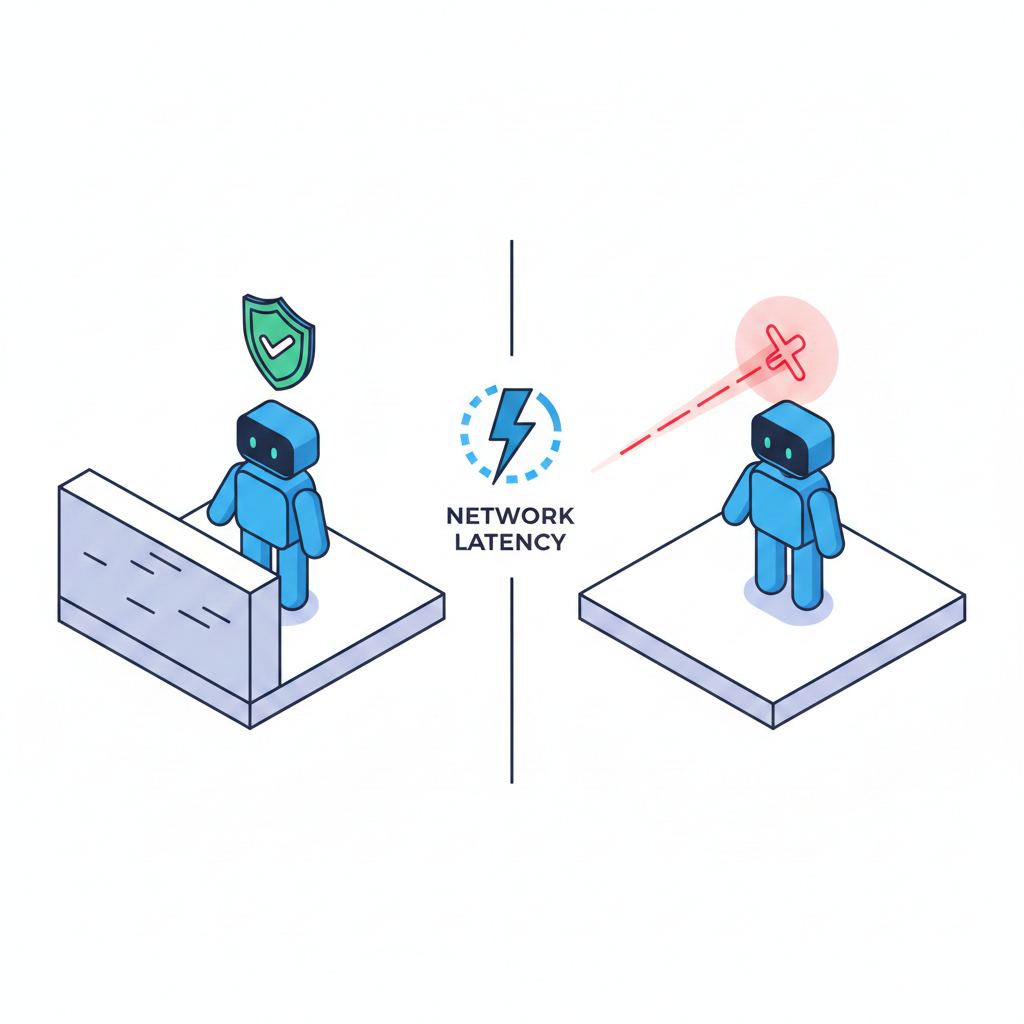
\includegraphics[width=1.0\linewidth]{figures/sec2/image1.png}
    \caption{视图一致性悖论：由于网络延迟（Latency），Client A 与 Client B 在同一物理时刻看到的“真相”截然不同。}
    \label{fig:network-lat}
\end{figure}

其次是\textbf{时序不确定性（Timing Uncertainty）}，指由于网络传输介质的物理特性，导致数据包到达的延迟（Latency）不可预知且次序（Ordering）可能错乱的现象。在单机代码中，函数调用的顺序就是逻辑执行的顺序，因果关系清晰可见。但在网络环境中，网络抖动（Jitter）和丢包（Packet Loss）会无情地打乱这一切。先发出的指令可能后到达，甚至根本不到达。如果服务器简单地按照“收到即执行”的原则处理，那么一场公平的决斗可能会变成比拼谁的网速更快，而不是谁的操作更准。更糟糕的是，如果两个玩家同时操作同一件物品，谁先谁后的判定将直接影响游戏结果。如何在一个异步的、不可靠的网络环境之上，构建一个逻辑上同步、时序上有序的虚拟时间轴，是所有网游后端必须解决的基础难题。

最后，也是最为致命的，是\textbf{信任边界（Trust Boundary）}，即在系统架构中划分出的安全隔离线，用于界定哪些计算节点是可被信任的，哪些是不可信且可能包含恶意行为的。单机游戏中，玩家拥有对自己机器的完全控制权，修改内存数据（如使用“金手指”或修改器）通常被视为个人娱乐行为，不会影响他人。但在竞技网游中，游戏客户端运行在充满恶意的不可控环境里。如果系统盲目信任客户端上报的数据——例如允许客户端直接汇报“我造成了1000点伤害”或“我现在瞬移到了终点”——那么外挂将摧毁整个游戏的公平性基石。玩家可能会通过篡改代码、拦截封包或修改内存来获得不当优势。因此，在线游戏不仅是技术的对抗，更是一场开发者与作弊者之间关于“真相定义权”的攻防战。

更进一步地，这种逻辑困境的普适性远超游戏领域。上述的三大挑战并非游戏所独有，而是所有“多端共享状态的实时在线系统”必须共同面对的工程公理。无论是金融领域中毫秒必争的高频交易系统，还是协同办公软件中多人同时编辑文档的冲突处理，亦或是元宇宙中海量并发的交互同步，其底层逻辑都受制于同样的分布式物理法则。只要系统涉及到多个物理分离的终端对同一个状态进行读写，就必然面临状态谁先谁后（时序）、各端看到的是否一样（视图一致性）以及恶意节点是否篡改数据（信任边界）的问题。多人在线游戏只不过是因为其对高频率交互和低延迟的极端苛刻要求，成为了这些分布式系统难题最集中的“试炼场”。

综上所述，从单机到联机，绝不仅仅是多加一个网络通信模块那么简单。它要求我们将思维模型从“维护一个确定的本地状态”彻底转变为“协调多个不一致的分布式状态”。在本章中，我们将不再把游戏世界视为封闭的本地进程，而是把它进化为一个需要“多终端共同维护”的在线系统。我们将聚焦于三个核心问题：\textbf{谁拥有世界的权威版本}（谁来定义唯一真相）、\textbf{本地视图如何围绕这一真相更新}（输入如何上传、结果如何下发）、以及\textbf{在存在不可信客户端时，哪些逻辑必须被收回到服务器一侧执行}。


% 发展的历史 怎么引入P2P
 
\subsection{初试锋芒：构建直连（P2P）对战原型} % <- 加入Socket编程 给一些代码 

在直面宏大的分布式架构之前，最符合工程师直觉的第一步往往是“奥卡姆剃刀”式的——既然只有两个玩家，为何不直接用一根网线将两台电脑连在一起？这种去中心化的直连模式（Peer-to-Peer, P2P），正是早期局域网联机游戏雏形。为了彻底理解网络同步的机理，我们不妨先动手构建这样一个最小化的 P2P 原型，亲身体验数据是如何跨越物理边界的。

构建这一原型的首要任务是建立通信通道。在操作系统的网络协议栈中，这一过程始于\textbf{套接字（Socket）}的创建。不同于单机程序直接读取内存，网络程序需要向内核申请一个“通信端点”。在双人直连模型中，我们需要人为地指定一方为“主机（Host）”，另一方为“客机（Guest）”。主机启动时会在本地绑定一个端口（Bind）并进入监听状态（Listen），就像是打开大门静候来客；而客机则知晓主机的 IP 地址与端口，主动发起连接请求（Connect）。经过 TCP 的三次握手建立起稳定的全双工通道后，两台物理隔离的计算机便在逻辑上拥有了共享的数据管道。此时，游戏循环（Game Loop）的逻辑发生了本质变化：每一帧的输入不再直接驱动本地逻辑，而是被分流为两路，一路进入本地缓冲区，另一路被序列化为二进制流，顺着网线飞向对手的缓冲区。

构建这一原型的核心挑战在于打破单机环境的封闭性，首要任务即是在操作系统网络协议栈中建立稳定的\textbf{套接字（Socket）}通信通道。网络程序不同于直接寻址内存的本地应用，它必须向内核申请一个逻辑上的通信端点，并通过 \textbf{IP 地址与端口号（Port）}这两大核心要素进行定位。IP 地址如同物理世界的门牌号，负责在复杂的网络拓扑中精确定位对手的计算机；而端口号则像是一座大厦中特定房间的编号，确保数据包能够准确送达对应的原型程序而非其他应用。通过将这两个参数封装进套接字，两台物理隔离的设备便具备了在逻辑层面上“感知”彼此存在的基础。

在具体的实现架构中，系统通过“主机（Host）”与“客机（Guest）”的身份划分来驱动连接。主机通过执行 Bind 操作将套接字与本地特定的端口绑定，随后进入 Listen 状态，在内核层面维持一个静默的监听队列。与此同时，客机携带主机的 IP 地址发起 Connect 请求，通过 TCP 协议标志性的“三次握手”建立起可靠的全双工数据链路。一旦这条逻辑管道贯通，底层游戏循环（Game Loop）的逻辑将发生本质演变：程序不再盲目处理本地输入，而是将每一帧的按键或指令序列化为二进制流，利用建立好的套接字实时外发。这意味着本地逻辑必须等待或预测来自远程缓冲区的数据，两台计算机由此在比特流的交换中达成了状态的同步

在\textbf{Go}语言中，Socket 编程可以通过标准库中的 \texttt{net} 包轻松实现。以下是一个简化的 P2P 连接建立示例：

\begin{tcolorbox}[title=P2P 连接建立示例]
\begin{lstlisting}[style=codeblock, language=go]
ln, err := net.Listen("tcp", "0.0.0.0:8080") // 用户A
conn, err := ln.Accept()
conn, err := net.Dial("tcp", "主机IP:8080") // 用户B
\end{lstlisting}
\end{tcolorbox}

连接建立后，玩家之间的数据交换便可通过读写 Socket 实现。例如，玩家A攻击了玩家B，玩家B的生命值下降了10点，这一信息需要被封装成数据包发送给对手：

\begin{tcolorbox}[title=数据包发送示例]
\begin{lstlisting}[style=codeblock, language=go]
// 发送数据
message := "DAMAGE:10"
conn.Write([]byte(message))
// 接收数据
buffer := make([]byte, 1024)
n, err := conn.Read(buffer)
receivedMessage := string(buffer[:n])
\end{lstlisting}
\end{tcolorbox}
同时，如果玩家B也进行了攻击，类似的消息会被发送回玩家A。通过这种双向的数据流，双方的游戏状态得以在各自的内存中更新。结合前述的游戏循环逻辑，玩家A在本地按下攻击键后，程序会先在本地内存中更新玩家B的生命值，然后将“DAMAGE:10”这一消息通过 Socket 发送给玩家B。给出\textbf{Go}语言的伪代码示例：
\begin{tcolorbox}[title=游戏循环中的数据交换示例]
\begin{lstlisting}[style=codeblock, language=go]
for {
    // 处理本地输入
    input := getLocalInput()
    synchronizeInput(input)
    // 处理接收的数据
    buffer := make([]byte, 1024)
    n, err := conn.Read(buffer)
    processReceivedData(buffer[:n])
}
\end{lstlisting}
\end{tcolorbox}


然而，如果玩家A和玩家B所处的网络环境比较差，导致数据包传输的延迟较高，游戏体验将大打折扣。玩家A在其屏幕上看到自己和玩家B的生命值都仅剩10点，玩家A进行极限操作攻击了玩家B，玩家B的生命值变为0，玩家A赢得比赛。但是玩家B也是在同一时间点看到的自己和玩家A的生命值都仅剩10点，玩家B也进行了极限操作攻击了玩家A，玩家A的生命值变为0，玩家B赢得比赛。最终导致双方都认为自己赢得了比赛，游戏逻辑陷入混乱。

为了保证双方在同一时间点对游戏状态有一致的认知，我们需要引入\textbf{时序同步机制}。在直连模式下，为了保证双方看到的一致性，我们通常采用“帧锁定（Lockstep）”策略。这就好比两个人下棋，必须遵循“你走一步，我走一步”的严格时序。在代码层面，我们将游戏时间切分为一个个离散的“逻辑帧（Turn）”。每一帧开始时，双方必须交换各自的输入指令（如“按下W键”或“点击鼠标”）。
程序会强制等待，直到本地输入和远端输入全部就位，才将这两组输入同时喂给游戏逻辑核心进行演算。
由于计算机的逻辑运算（如果是确定性的）在输入相同的情况下必然产生相同的结果，
只要保证两端收到的输入序列完全一致，两台电脑上的游戏世界就会像精密咬合的齿轮一样同步运转，
无需传输庞大的全量状态数据。

加入帧锁定机制后的伪代码示例如下：
\begin{tcolorbox}[title=帧锁定机制示例]
\begin{lstlisting}[style=codeblock, language=go]
for {
    // 收集本地输入
    localInput := getLocalInput()
    conn.Write([]byte(localInput))

    // 等待接收远端输入
    buffer := make([]byte, 1024)
    n, err := conn.Read(buffer)
    remoteInput := string(buffer[:n])
    // 同步处理输入
    processInputs(localInput, remoteInput)
}
\end{lstlisting}
\end{tcolorbox}
通过这种方式，双方在每一帧都能基于相同的输入序列计算出一致的游戏状态。

当然，我们还希望能保存角色的位置、血量等状态，以便在断线重连时恢复游戏进度，总不能让玩家每次断线都从头开始吧？为了方便起见，我们可以在每次游戏状态更新后，将当前的全量状态序列化并保存到本地文件中。当玩家重新连接时，程序可以读取这个文件，恢复到上次保存的状态，从而实现断线重连功能。

然而，当我们试图将这个看似完美的 P2P 原型搬上广域网时，现实的引力便会将其击碎。
首先是\textbf{流畅度与公平性的博弈}。在帧锁定机制下，游戏的推进速度取决于网络状况最差的那一端，
一旦一方发生网络抖动，另一方的画面也会随之冻结，这种“一人卡顿，全场遭殃”的体验在互联网环境下是致命的。
更严峻的是\textbf{信任危机}。在 P2P 架构中，必定有一方（通常是主机）承载了部分逻辑裁决权，
或者双方各自计算。这就给作弊者留下了巨大的后门：如果玩家 A 修改了本地内存中的判定逻辑（
例如将命中判定范围扩大），玩家 B 的机器要么被迫接受这个错误结果，要么检测到状态不一致导致游戏崩溃（Desync）。

正是这次构建 P2P 原型的尝试，让我们痛切地意识到：在缺乏可信第三方监督、且网络环境不可控的互联网上，
单纯的直连与协商机制极其脆弱。
为了解决“谁说了算”以及“如何不被卡顿拖累”这两个核心痛点，
我们必须打破平等的 P2P 拓扑，引入一个绝对权威的仲裁者。这，便是下一节 CS 架构登场的契机。

\subsection{中流砥柱：CS架构和双人原型} % <- 发展到CS
% <- 一个简单能够接受长连接的S怎么写 -> 轮询
% 现在大家已经知道服务器的特点，那么适用于原型的怎么写呢 并发 并发是两个 
% 同步的锁给个代码 

基于前文分析，虽然P2P架构在《星际争霸1》等早期局域网时代的经典之作中表现优异，凭借“帧同步”与“确定性模拟”实现了低带宽下的高效同步，但这一模式本质上建立在“协作信任”与“高质网络”的假设之上。一旦置身于环境复杂的广域网（WAN），面对网络抖动与人性幽暗，P2P架构便会暴露出其致命的软肋——不仅难以彻底根除作弊，更面临着“一人卡顿，全场等待”的木桶效应。因此，为了构建一个能够适应现代互联网环境、且具备强壮性的双人在线系统，引入一个独立于所有玩家之外的第三方节点，即经典的CS架构（Client-Server Architecture），便成为了必然的进化方向。

\begin{figure}[H]
    \centering
    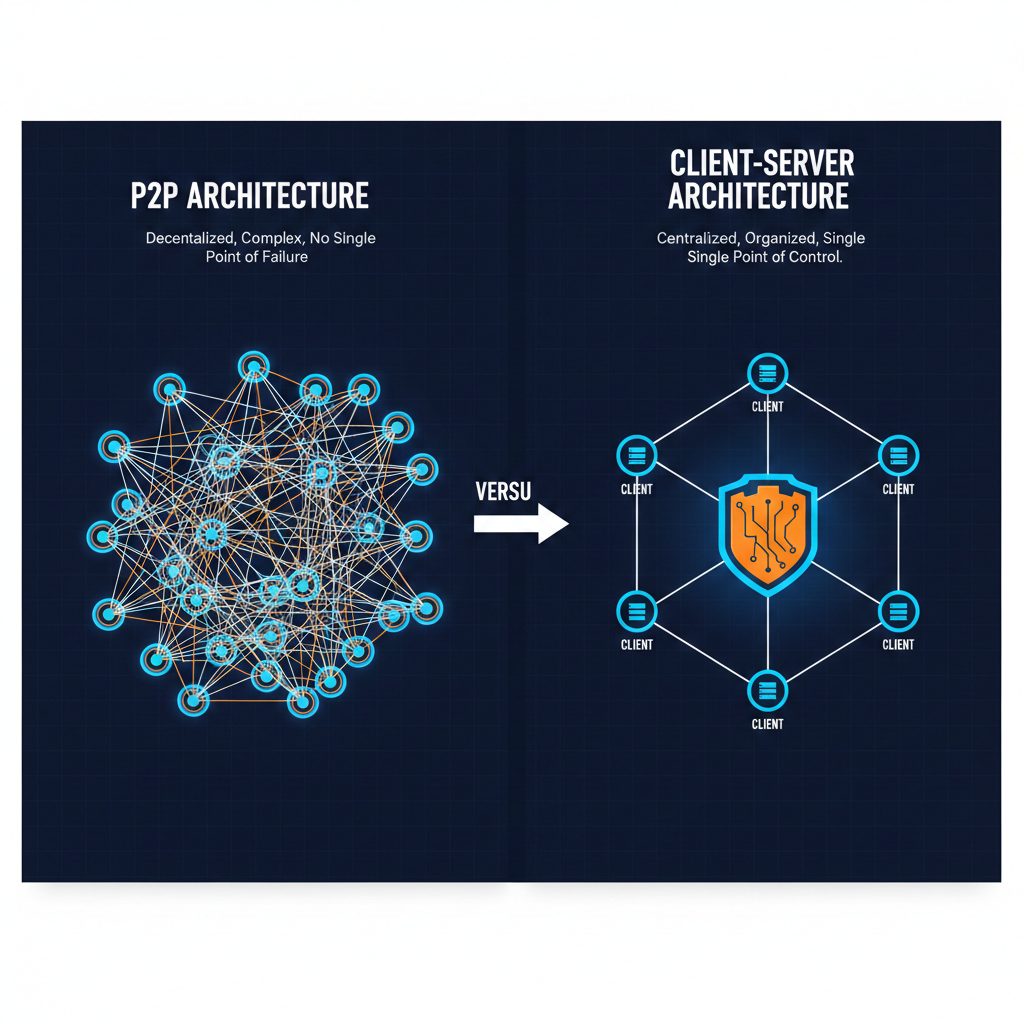
\includegraphics[width=1.0\linewidth]{figures/sec2/image2.png}
    \caption{架构演进：左图为 P2P 全状/网状结构，依赖相互信任；右图为 CS 星型结构，服务器（Server）作为唯一权威节点。}
    \label{fig:p2pvscs}
\end{figure}

在这种架构范式下，核心的变革在于引入了\textbf{权威服务器（Authoritative Server）}这一概念。它绝非仅仅是一个负责转发数据包的中转站，而被定义为\textbf{“游戏世界状态的唯一合法持有者”}。在物理层面，它独立于所有客户端运行；在逻辑层面，它拥有对游戏规则的最高解释权与裁决权。任何客户端计算出的结果——无论是角色的位移、子弹的弹道还是技能的释放——在本质上都仅仅被视为一种“请求”或“本地表现”。唯有经过服务器校验、计算并确认的数据，才是不可篡改的“世界真相”。

我们之所以在本系统中坚定地选择CS架构而非P2P，其深层逻辑在于对\textbf{“信任模型”}的重构。P2P架构更适用于小规模、高频交互且对延迟极度敏感的场景（如局域网联机或格斗游戏），因为它默认参与者之间存在较高的信任度，且网络环境可控。然而，一旦游戏场景涉及强对抗性（Anti-cheat）、持久化资产（如经济系统或装备存档）或是大规模连接，客户端便不再可信。此时，CS架构通过“零信任”原则，强制将计算权收归服务端，虽然这不可避免地牺牲了部分响应速度（RTT），但却换取了整个系统的安全性与一致性。简而言之，当游戏从“协作体验”转向“竞争博弈”时，架构必须从P2P的“多方共识”转向CS的“独裁仲裁”。

这种权力的转移，直接导致了客户端角色的\textbf{降维}与输入模式的\textbf{重构}。在CS架构中，客户端从全知全能的“主宰”退化为了一个高级的“哑终端”。它不再负责核心逻辑的推演，而是专注于交互意图的采集与画面的渲染表现——即“逻辑与表现的分离”。当玩家按下键盘上的“W”键时，客户端无权直接修改角色的坐标，它只能将这个“移动意图”封装成数据包发送给服务器。此时屏幕上的角色移动，在逻辑上仅仅是对服务器未来状态的一种“预测”或对已确认状态的“回放”。

这一机制的优越性，将在我们即将构建的双人追逐战原型中得到淋漓尽致的体现。设想若没有权威服务器，当玩家A声称抓住了玩家B，而B声称已逃脱时，系统将陷入无解的罗生门。而在权威服务器模式下，流程被重塑为：玩家A上传“攻击操作”；服务器基于内存中维护的权威坐标进行距离校验与逻辑运算；若判定有效，服务器更新状态并广播结果。此时，即便玩家B试图通过本地外挂锁定血量，或者因网络延迟看到了错误的位置，一旦收到服务器下发的权威快照，他的客户端必须无条件地执行状态回滚（Reconciliation），修正本地数据以符合服务器的裁决。这便是“权威性”的核心价值所在。

为了验证这一理论，我们将摒弃商业引擎的图形干扰，从零构建一个“双人原型”。
在这个原型中，服务器将是一个运行在控制台的纯逻辑进程，它看不见任何图形，只处理坐标数值、状态枚举与伤害公式；
而客户端则负责将玩家操作转化为网络流，并将服务器下发的抽象数据流转化为屏幕上的红蓝方块。

首先我们将前文的伪代码结构进行调整，以适应CS架构的需求：
\begin{tcolorbox}[title=CS架构伪代码结构,label=code:cs_structure]
\begin{lstlisting}[style=codeblock, language=go]
for {// 服务器端主循环
    // 接收客户端输入
    inputA := receiveInputFromClientA()
    inputB := receiveInputFromClientB()
    // 处理游戏逻辑
    updateGameState(inputA, inputB)
    // 广播权威状态
    broadcastState()
}
for { // 客户端主循环
    // 采集本地输入
    localInput := getLocalInput()
    sendInputToServer(localInput)
    // 接收权威状态
    gameState := receiveGameStateFromServer()
    renderGameState(gameState)
}
\end{lstlisting}
\end{tcolorbox}

从上面的结构可以看出，服务器端的主循环负责接收来自两个客户端的输入，处理游戏逻辑，
并将更新后的权威状态广播回各个客户端；而客户端则专注于采集本地输入、发送给服务器，
并渲染服务器下发的权威状态。这就可以确保所有玩家可以看到一致的游戏世界，解决了前文提到的\textbf{视图一致性}问题。



\subsection{运筹帷幄：连接管理、状态仲裁以及世界同步}

在确立了以服务器为中心的架构范式后，我们需要透过宏观的拓扑结构，深入拆解服务器内部微观的运作机理。
一个成熟的后端系统，绝非仅仅是一个被动接收并转发比特流的数据中转站，而应当是一个拥有高度自主权、
时刻处于高速逻辑运算中的“大脑”。

在我们的双人对战原型乃至更复杂的分布式系统中，这个“大脑”的运转逻辑被严谨地解构为三个相互依存的核心模块：
\textbf{连接管理（Connection Management）}、\textbf{状态仲裁（State Arbitration）} 以及 
\textbf{世界同步（World Synchronization）}。这三者分别对应了分布式计算中的资源生命周期维护、
数据一致性保障以及状态分发机制，共同构成了在线业务后端的最小完备闭环。


\begin{figure}[H]
    \centering
    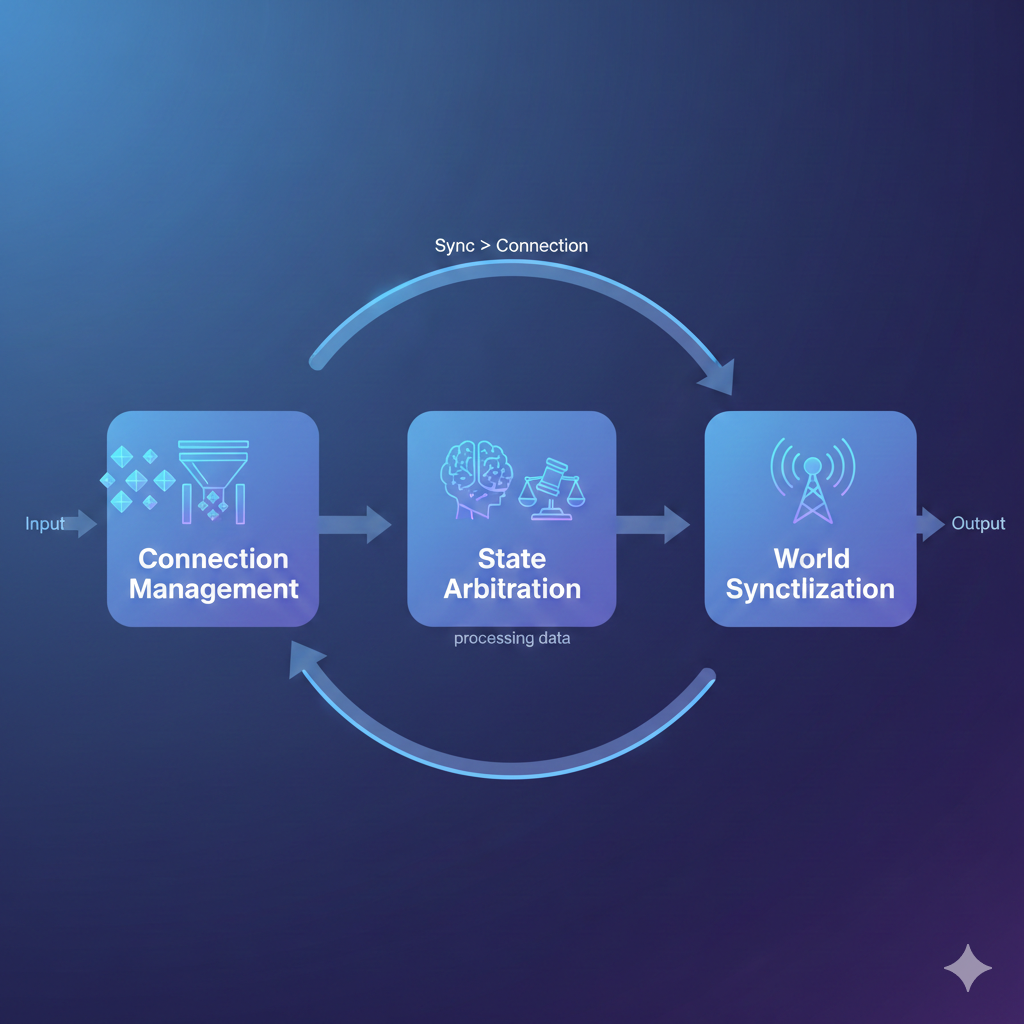
\includegraphics[width=1.0\linewidth]{figures/sec2/image3.png}
    \caption{服务器逻辑闭环：数据经由“连接管理”流入，在“状态仲裁”层进行逻辑校验与更新，最终通过“世界同步”广播回客户端。}
    \label{fig:csmodules}
\end{figure}
\subsubsection{连接管理：会话的生命周期守护与资源调度}

连接管理是任何长连接服务的门户与基石。在通用的分布式系统语境下，它的核心职责在于\textbf{“资源的动态分配与上下文维护”}。无论是即时通讯软件、金融交易终端还是网络游戏，服务器必须在不可靠的物理网络之上，抽象出一个可靠的逻辑会话层，以确保每一个接入终端都能被精确地标识、追踪与管理。

在游戏服务器的具体实现中，连接管理的角色远超底层的 TCP Socket 握手。它首先承担着“守门人”的重任，负责在传输层之上构建应用层的准入机制。当客户端发起连接请求时，管理模块必须执行严格的合法性校验（例如 Token 验证或加密握手），以过滤掉无效的扫描流量或恶意的 DDoS 攻击尝试。

一旦连接建立，服务器随即进入资源调配阶段，为该客户端分配全局唯一的会话 ID（Session ID），并在内存堆中开辟一块专用的上下文区域（Context）。这块区域不仅存储着玩家的网络句柄，还承载着序列号管理、拥塞控制窗口以及断线重连所需的快照数据。

更为关键的是，连接管理模块必须具备极高的鲁棒性来应对移动网络环境的波动。它通过精密的\textbf{心跳检测机制（Heartbeat）}与\textbf{超时策略}，敏锐地量化连接的健康度，从而区分正常的“用户静默”与异常的“网络掉线”。针对游戏场景中常见的网络抖动，成熟的管理模块不会在检测到断开的瞬间立即销毁数据，而是通过引入“会话保持期（Session Persistence）”或“影子状态”，允许客户端在特定时间窗口内通过重连协议无缝恢复上下文。这种设计既避免了因网络瞬断导致的频繁登出，也确保了在用户彻底离开时能通过回调机制优雅地释放内存，防止因“僵尸连接”堆积而引发生的资源泄露危机。

在完善了基础网络框架后，我们需要对 \ref{code:cs_structure} 中的输入处理逻辑进行升级。
为了解决裸连接（Raw Connection）难以维护状态的问题，我们引入 clientConn 结构体。
它将底层的网络连接与玩家的业务属性（如会话 ID、心跳时间、事件队列）封装在一起，实现标准化的连接管理。

\begin{tcolorbox}[title=连接管理的结构体定义] 
\begin{lstlisting}[style=codeblock, language=go]
type clientConn struct { 
    id int // 唯一会话标识 
    Conn net.Conn // 底层 TCP/UDP 连接 
    lastHeartbeat time.Time // 最后心跳时间，用于超时检测 
    EventQueue chan InputEvent // 输入事件缓冲通道 
}
// 实例化客户端连接对象 
var clientA clientConn 
var clientB clientConn
\end{lstlisting} 
\end{tcolorbox}

然后我们会使用上面定义过的结构体，来处理并管理请求。


\begin{tcolorbox}[title=连接管理伪代码示例]
\begin{lstlisting}[style=codeblock, language=go]
func handleConn(client *ClientConnection) {
    for { // 读取数据
        input, err := receiveInputFromClient(client.Conn)
        if err != nil { // 处理断线或错误
            handleDisconnect(client)
            return
        }
        client.LastHeartbeat = time.Now() // 更新心跳时间
        client.EventQueue <- input  // 将输入放入事件队列
    }
}
go handleClientConnection(&clientA)
go handleClientConnection(&clientB)
tiker := time.NewTicker(tikeoutDuration)
for { // 从事件队列中获取输入
    select {
    case <- tiker.C: // 检测超时
        checkAndHandleTimeout(&clientA)
        checkAndHandleTimeout(&clientB)
    }
    updateGameState()  // 处理游戏逻辑
    broadcastGameStateToClients() // 广播权威状态
}
\end{lstlisting}
\end{tcolorbox}

此时，连接管理模块已经能够高效地维护每个客户端的会话状态，整个游戏的进程不会因为单个连接的波动而受到影响。
并且，通过划分每帧的输入处理与超时检测，我们在一定程度上缓解了网络抖动对游戏体验的冲击，解决了\textbf{时序不确定性}的问题。


\subsubsection{状态仲裁：逻辑的一致性防线与真理裁决}

状态仲裁是服务器架构中“权威性（Authority）”的集中体现。在广泛的软件工程领域，这对应着\textbf{“单一数据源（Single Source of Truth）”}与\textbf{“业务逻辑校验”}的核心原则。在一个互不信任的客户端-服务器网络环境中，永远不能假设接入端的输入是诚实或正确的，因此服务器必须作为唯一的真理裁决者，对所有状态变更请求进行审计与执行。

在激烈的双人对战中，每秒钟可能会有海量的操作指令——从移动向量到技能触发——如潮水般涌向服务器。仲裁模块决不会盲目地根据客户端的指令更新状态，而是构建了一套严密的\textbf{“先校验，后执行”}的流水线体系。

以空间位置更新为例，当服务器接收到移动请求时，并不会直接采信客户端上报的目标坐标，
而是引入物理引擎或碰撞检测算法进行逻辑复核：系统会根据上一帧的权威位置、
时间差以及角色的最大理论速度，计算出合理的移动包络线。只有当请求落在这个合法范围内，
且未穿越不可逾越的地理屏障（NavMesh）时，该操作才会被标记为有效。同理，在处理战斗交互时，
仲裁模块会完全忽略客户端上报的“命中结果”，转而依据服务器端记录的时间切片和空间状态，
重新进行一次权威的判定。通过这种严苛的过滤机制，服务器彻底杜绝了诸如加速、穿墙或篡改数据等作弊行为，
确保了所有参与者都在同一套不可被逾越的规则下进行公平竞技。

为了将状态仲裁的逻辑融入到 \ref{code:cs_structure} 中的游戏逻辑处理部分，我们可以修改如下：
\begin{tcolorbox}[title=状态仲裁伪代码示例]
\begin{lstlisting}[style=codeblock, language=go]
func processInputFromClientA(input InputEvent) {
    // 校验输入合法性
    if isValidInput(input, playerA.State) {
        // 更新玩家A状态
        updatePlayerState(&playerA, input)
    } else {
        log.Println("Invalid input from Client A:", input)
    }
}
func processInputFromClientB(input InputEvent) {
    // 校验输入合法性
    if isValidInput(input, playerB.State) {
        // 更新玩家B状态
        updatePlayerState(&playerB, input)
    } else {
        log.Println("Invalid input from Client B:", input)
    }
}
\end{lstlisting}
\end{tcolorbox}

此时，状态仲裁模块已经能够有效地过滤掉异常或恶意的输入请求，确保游戏逻辑的纯净性与一致性，解决了\textbf{信任边界}的问题。

然而，仅有仲裁还不够——服务器内存中的权威状态是易失的。一旦服务器进程重启或玩家断线，内存中的角色坐标、生命值等数据将随之消失。如果每次断线都让玩家从零开始，游戏体验将无从谈起。因此，我们需要在状态仲裁的基础上引入持久化机制，将关键的玩家状态定期写入磁盘存储。

持久化的位置选择同样遵循信任边界原则。如果将存档保存在客户端本地，玩家可以轻易篡改存档文件来伪造属性；而将存档保存在服务器端的数据库中，则能确保数据的权威性与完整性。在我们的双人原型中，选择SQLite作为轻量级的嵌入式数据库——它无需独立的数据库服务进程，只需一个本地文件即可运行，非常适合教学原型的快速验证。

具体而言，我们定义一个存储接口，将玩家的核心状态（名称、坐标、生命值）抽象为可持久化的记录：

\begin{tcolorbox}[title=持久化存储接口]
\begin{lstlisting}[style=codeblock, language=go]
type StoredPlayer struct {
    Name string
    X, Y int
    HP   int
}

type Store interface {
    LoadPlayer(name string) (*StoredPlayer, error)
    SavePlayer(p StoredPlayer) error
}
\end{lstlisting}
\end{tcolorbox}

每当状态仲裁模块完成一次合法的状态变更（如移动校验通过、战斗结算完毕），服务器便调用\texttt{SavePlayer}将最新状态写入数据库。这里采用``INSERT ... ON CONFLICT DO UPDATE''（即UPSERT）语义，确保无论玩家是首次登录还是已有存档，都能用一条语句完成写入。当玩家断线后重新连接时，服务器在注册阶段调用\texttt{LoadPlayer}，若数据库中存在该玩家的记录，则以存档数据恢复其坐标与生命值，而非重新随机生成。

需要指出的是，当前原型在每次状态变更后都立即执行数据库写入，这种同步持久化方式在双人场景下完全可行，但在高并发场景下会因频繁的磁盘I/O成为性能瓶颈。第三章将引入Redis内存缓存与异步写回策略来解决这一问题。
\subsubsection{世界同步：状态的最终一致性与高效分发}

世界同步模块负责闭合信息流动的环路，将服务器内部经过仲裁的权威结果反馈给所有参与者。在分布式计算理论中，这属于\textbf{“状态复制（State Replication）”}与\textbf{“发布/订阅（Pub/Sub）”}模式的范畴。其核心挑战在于如何在有限的网络带宽与高频的实时性要求之间找到平衡点，以实现系统状态的\textbf{“最终一致性”}。

服务器维护的真理如果仅停留在内存中，对于玩家而言便是毫无意义的黑盒。因此，同步模块需要以固定的高频率（即 Tick Rate，如 30Hz 或 60Hz）驱动整个世界的演变，并将每一帧内的状态变更——包括位置迁移、属性增减、动画状态切换等——转化为数据流广播出去。

这一过程不仅是数据的搬运，更是复杂的工程权衡艺术。为了避免全量数据广播带来的带宽风暴，现代同步模块广泛采用\textbf{“增量同步（Delta Synchronization）”}与\textbf{“快照（Snapshot）”}相结合的混合策略。对于初次进入视野的实体，系统发送包含完整状态的全量快照；而对于已存在于上下文中的实体，则仅发送自上一帧以来发生变化的属性差值。此外，为了进一步压榨传输效率，还需要引入 Protocol Buffers 或 FlatBuffers 等高效序列化技术，将结构化对象压缩为紧凑的二进制流。当客户端接收到这些权威数据包后，结合本地的插值（Interpolation）与预测（Prediction）算法，便能平滑地渲染出连续的画面，从而在玩家的感官层面构建出一个与对手实时互动、毫无违和感的统一时空。

为了将世界同步的逻辑融入到 \ref{code:cs_structure} 中的广播权威状态部分，我们可以修改如下：
\begin{tcolorbox}[title=世界同步伪代码示例]
\begin{lstlisting}[style=codeblock, language=go]
func broadcastGameStateToClients() {
    // 构建增量状态包
    deltaStateA := constructDeltaState(playerA, lastSentStateA)
    deltaStateB := constructDeltaState(playerB, lastSentStateB)
    // 发送给客户端A
    sendGameStateToClient(clientA.Conn, deltaStateA)
    // 发送给客户端B
    sendGameStateToClient(clientB.Conn, deltaStateB)
    // 更新上次发送状态
    lastSentStateA = playerA.State
    lastSentStateB = playerB.State
}
\end{lstlisting}
\end{tcolorbox}

\subsubsection{合璧成环：三模块的协同闭环}

通过上述三个模块的精密咬合——连接管理维持通信通道的稳定性，状态仲裁确立逻辑事实的唯一性，世界同步保障感知层面的实时性——我们的双人对战原型便拥有了完整的生命力。这一架构不仅解决了基础的联机互通需求，更在底层设计上预置了针对网络延迟（Latency）的容错能力与针对恶意行为（Cheating）的免疫能力，为后续章节中探讨大规模并发（Concurrency）与更复杂的战斗逻辑奠定了坚不可摧的标准范式。

%%

\subsection{狭路相逢：双人对战流程全景}


在前两节的论述中，我们分别从系统架构的宏观视角和模块职责的微观维度，详细阐述了双人在线原型的设计思路：服务器作为绝对的权威仲裁者，全权负责网络连接管理、全局状态仲裁以及世界状态的同步；而客户端则专注于用户输入的实时采集与游戏画面的渲染展示。为了更具体地展示这一架构在实际运行中的动态表现，本节将打破静态的模块划分，沿着一场标准对战的时间轴线，从玩家相遇、交互发起到胜负裁决的完整生命周期，从全链路的整体视角深度梳理前述机制是如何协同工作的。这不仅是对功能的串联，更是对“权威服务器”设计模式在时序逻辑上的具体印证。

\subsubsection{对战前阶段：相遇与可见性建立}

在对战尚未触发的自由探索阶段，服务器不仅维护着所有在线玩家的坐标数据，更在每一个逻辑帧中基于权威坐标执行严格的空间查询与可见性计算。系统会根据预设的感兴趣区域（AOI, Area of Interest）算法，动态判断实体间的拓扑关系。对于任意一对玩家，当其中一方的坐标进入另一方的视野半径时，服务器会首先在内存中更新双方的视野列表（View List），随后在接下来的状态同步周期中，将这一新增的实体信息序列化并打包进下行数据包。

客户端在接收到数据包并反序列化后，会在本地场景图中实例化对应的角色模型，玩家侧由此感知到“地图上出现了一名新对手”。在此过程中，必须强调的是，所有的可见性判断——即“谁能看见谁”——完全由服务器基于其内存中的权威状态独立完成。客户端仅作为被动的接收端，负责将服务器下发的逻辑状态“翻译”为视觉图像。这种单向的数据流设计，确保了在网络波动或客户端被篡改的情况下，全局的可见性关系依然保持逻辑上的严密统一，彻底杜绝了客户端预判导致的“幽灵玩家”或视野状态不同步的割裂现象。

\subsubsection{对战发起：资格判定与会话原子性}

当玩家之间建立了可见关系后，系统并未立即进入战斗状态，而是需要进行更细粒度的条件校验。随着两名玩家的距离进一步缩短并触及预设的交战阈值，服务器会在内存状态机中将双方标记为“潜在可交互”状态，并通过轻量级的状态位更新通知客户端。客户端 UI 层据此激活交互控件，向玩家展示“可以发起对战”的视觉提示。此时，尽管界面上允许操作，但这一提示仅代表一种客户端的本地预测，并未对服务器端的逻辑状态产生任何实质性变更。

一旦某位玩家触发对战请求，客户端会将该操作意图编码为特定的请求消息（Request）发送至服务器。服务器在接收到该请求后，绝不会盲目响应，而是基于当前这一帧的最新权威数据进行一次严格的原子性校验：重新计算双方距离是否仍在合法范围内、确认双方是否仍处于空闲状态、以及检查是否涉及第三方冲突。这一过程类似于数据库事务的隔离性检查，只有当所有前置条件在当前逻辑帧内同时满足时，服务器才会通过校验，在内存中实例化一个对战会话（Session）对象，并将两名玩家的状态机从“自由移动”原子性地切换至“对战锁定”。随后的状态同步将这一确定性的状态变更广播回客户端，从而将界面上的操作意图转化为服务器端受管理的正式会话。

\subsubsection{战斗过程：确定性裁决与逻辑投影}

为了最大限度地凸显服务器端权威判定的核心价值，本书有意选取了一种极简的单回合对战模型作为首个原型，暂时剥离了复杂的技能树与即时演算系统。在这一高抽象度的模型中，战斗过程本质上是一次由服务器主导的确定性计算：在特定的逻辑帧上，服务器锁定双方状态，读取关键属性，依据统一算法产出唯一结果，并写入权威数据。

具体而言，当流程进入裁决阶段，服务器会从持久化层或内存缓存中调取两名玩家的基础战力、当前生命值及所有生效的增益状态。原型实现采用了一套标准的数值对抗公式——例如以战力差值为基准，引入受控的伪随机数序列作为扰动因子——从而计算出不可辩驳的胜负判定。紧接着，服务器在同一逻辑线程内执行状态更新（State Update）：胜方获得经验积累，败方扣除生命值。整个过程是一个严格的黑盒计算，完全不依赖客户端的任何输入或本地运算结果。即便恶意客户端通过内存修改在本地伪造了“暴击”或“闪避”的视觉效果，由于这些数据从未参与服务器端的逻辑运算，因此无法对最终的权威裁决产生丝毫影响。这一设计贯彻了网络游戏开发的核心铁律：客户端仅负责请求的发起与结果的视觉投影，而所有涉及游戏性（Gameplay）的逻辑演算必须在权威服务器的安全边界内闭环。

\subsubsection{对战结算：状态一致性与分布式事务}

当胜负结果被写入权威状态后，系统进入生命周期的最后阶段：结算同步与世界状态回退。这一过程在逻辑上等同于一次分布式事务的提交与连接释放。首先，服务器构建包含胜负判定、属性变更增量及后续状态指令的结算数据包，并下发给相关客户端。客户端解析后，驱动 UI 弹出结算面板并播放相应的胜负动画。需要注意的是，客户端展示的数值变化完全是服务器数据的副本，客户端本地绝不执行任何属性的加减运算。

与此同时，服务器执行逻辑状态的回退操作（Rollback），将两名玩家从独占的“对战会话”中解耦，并在同一逻辑帧内将他们的状态机重置为“自由移动”模式，重新纳入常规的大世界同步循环。在随后的广播周期中，周围的其他玩家将基于新的全局状态，观察到这两名角色结束了战斗状态或发生了位置变更。至此，一个包含相遇检测、会话建立、逻辑裁决及状态重置的完整闭环在服务器端严丝合缝地执行完毕，并在客户端侧呈现为一段连贯流畅的游戏体验。

\subsubsection{从游戏到分布式系统：本质的统一}

跳出具体的游戏场景，若我们将视角上升至分布式系统架构的高度，会发现上述的双人对战流程本质上是一个典型的 \textbf{状态机复制（State Machine Replication）} 与 \textbf{中心化一致性（Centralized Consistency）} 问题的工程实践。

在这个模型中，服务器扮演着 Leader 或 Coordinator 的角色，维护着系统的单一真值（Source of Truth）；而所有的客户端则是分布在不同网络节点的 Follower 或 Replica。玩家的操作不再仅仅是游戏指令，而是向协调者发起的远程过程调用（RPC）或事务请求。服务器对“相遇”的判定对应着分布式系统中的邻居发现与拓扑维护；“对战发起”时的资格校验，实则是为了防止竞态条件（Race Condition）而设置的分布式锁或乐观并发控制；而“战斗裁决”则是事务的具体执行逻辑，确保了在不可靠的网络环境下，系统状态（如玩家血量、积分）变更的原子性（Atomicity）与一致性（Consistency）。通过这种架构，我们解决的不仅仅是游戏玩法的同步，更是如何在存在网络延迟和不可信节点的分布式环境中，保证系统全局状态有序演进这一核心计算机科学难题。

\subsubsection{流程总结}

为了更直观地理解这一涵盖了网络通信、逻辑运算与状态管理的复杂交互过程，我们将上述从相遇、就绪、裁决到结算的完整时序绘制成图~\ref{fig:battle_flow}。从图中可以清晰地看到，客户端与服务器被网络边界严格隔开：尽管客户端承载了复杂的画面表现和用户交互，但所有跨越网络边界的关键指令——无论是视野的判定（Visibility）、状态的流转（State Transition）还是胜负的产生（Arbitration）——其逻辑闭环始终收敛在权威服务器内部，客户端仅仅是这一权威逻辑的“投影仪”。

\begin{figure}[htbp]
    \centering
    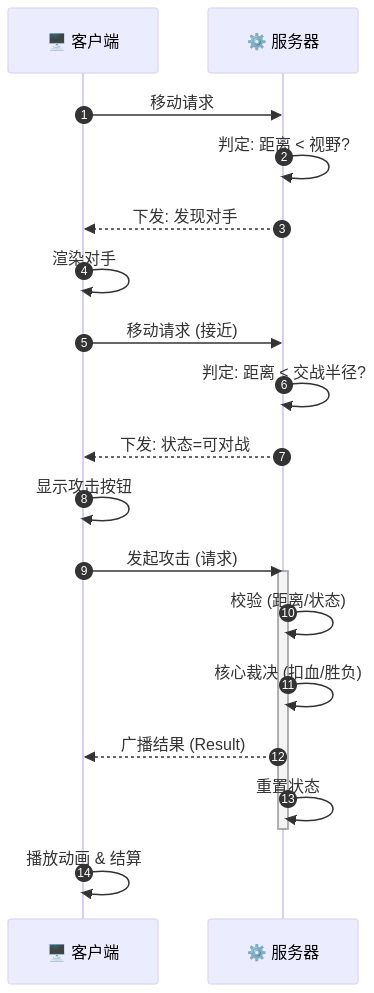
\includegraphics[width=0.45\linewidth,keepaspectratio]{figures/battle_flow.png}
    \caption{整体流程}
    \label{fig:battle_flow}
\end{figure}

回顾本章开头提出的三类挑战，可以看到：视图一致性通过服务器统一维护可见关系与世界同步来保障；时间与顺序问题通过集中化的请求校验和单线程裁决来化解；而信任边界则通过将关键逻辑彻底收拢到服务器一侧而得到收紧。本节给出的双人对战流程，为后续在并发规模和地图数量进一步扩展时的系统演化，提供了一个清晰可依的基本形态。

\subsection{小结：双人原型的确立与并发时代的前夜}

至此，我们不仅完成了一个双人对战原型的构建，更重要的是确立了网络游戏开发中至关重要的认知里程碑：构建在线世界的核心，在于搭建由\textbf{连接管理}、\textbf{逻辑仲裁}以及\textbf{状态同步}所构成的最小闭环。在这个闭环中，我们剥离了单机时代的思维惯性，确立了一条不可逾越的铁律——服务器是唯一的权威熵源，它只负责产出不可辩驳的\textbf{结果}；而客户端则退化为表现层，它只负责上报玩家的\textbf{意图}并如实呈现服务器下发的结论。这种“意图上报”与“结果下发”的异步循环，正是所有多人在线交互系统的基石。

回顾本章历程，我们正是基于上述理论，完成了从单机思维向在线思维的第一次系统性跨越。在单机模式下，世界被封闭在本地进程的孤岛中，内存状态即是真理；而一旦引入网络，多端数据的不一致性迫使我们必须划定明确的信任边界。为此，我们引入了经典的 CS (Client-Server) 架构作为解决方案：将服务器定义为无渲染的纯逻辑实体，它在内存中维护着唯一的“世界真相”。通过双人对战这一具象场景，我们演示了服务器如何作为连接中介管理会话，如何作为状态管理者收敛数据，以及如何作为逻辑仲裁者处理移动与攻击指令。在这个体系下，任何本地计算都仅仅是对未来的预测，只有服务器的裁决才是最终的历史。

然而，从工程演进的视角审视，目前的成果依然是一个“教学友好”的温室模型。我们的世界目前仅容纳两名玩家，且服务器逻辑严格遵循单线程的时间线顺序执行。在微观的低负载环境下，这种简单的请求-响应模型足以维持世界的运转；但一旦我们将视野投向宏观的真实环境——当成百上千名玩家挤入同一张地图，海量的登录、移动与战斗请求将如洪水般涌入单一的逻辑通道。

此时，简单的顺序处理将瞬间成为性能的瓶颈，任何微小的阻塞都会被放大为全局的停滞。更严峻的是，当多名玩家同时争抢同一份资源或修改同一组数据时，缺乏并发控制的系统极易陷入数据竞争与状态错乱的深渊。因此，接下来的第三章将是工程实践的又一次飞跃。我们将引入 Go 语言强大的并发原语 (Goroutine)，打破顺序执行的枷锁，让服务器具备同时处理成千上万个并发连接的能力；同时，我们将引入锁与同步机制来应对高并发带来的复杂性挑战。如果说本章解决了“为什么需要服务器”的定性问题，那么下一章将致力于解决“如何让服务器在洪峰压力下依然稳如磐石”的定量难题。

\newpage    